\documentclass[11pt]{article}
\usepackage[colorlinks,urlcolor=blue]{hyperref}
\usepackage{graphicx}

\topmargin 0in
\textheight 8.75in
\textwidth  5.75in

\parskip 5pt


\begin{document}

\title{OP2 Developers Guide - Distributed Memory (MPI) Parallelisation}
\author{Gihan R. Mudalige and Mike Giles}

\maketitle

\begin{abstract}
\noindent This document explains OP2's distributed memory parallelisation design and implementation based on MPI.  It is
intended primarily for those who are developing OP2 for distributed memory multi-core CPU and/or GPU clusters and should
be read in conjunction with the OP2 developer manual for single node systems. Those who are only using OP2 should
instead read the Users Manual.
\end{abstract}

%\newpage




\tableofcontents

\newpage

\section{Introduction}
The OP2 design uses hierarchical parallelism with two principal levels. At the highest level, OP2 is parallelised across
distributed-memory clusters using MPI message-passing.  This uses essentially the same implementation approach as the
original OPlus~\cite{oplus}.  The domain is partitioned among the compute nodes of the cluster, and import/export halos
are constructed for message-passing.  Data conflicts when  incrementing indirectly referenced datasets are avoided by
using an ``owner-compute'' model, in which each process performs the computations which are required to update data
owned by that partition.  The second level of parallelisation is achieved within a single multi-core CPU or GPU node.
The multi-CPU parallelisation is currently supported by OpenMP threads and in the future will support other techniques
such as Intel's AVX. The GPU support is based on NIVIDIA CUDA and will later support OpenCL. The single node design and
implementation is the subject of the OP2 developer manual. In this document we detail the design of the distributed
memory level based on MPI and describe some of its key implementation aspects. We also detail the heterogeneous cluster
back-end design which facilitates the development and execution of an OP2 application on a cluster of GPUs and a
cluster of multi-threaded CPUs. The Airfoil example application supplied with the OP2 release is used as an example to
illustrate the design and implementation.




\section{MPI parallelisation strategy}
% parallel start-up
\subsection{Parallel Startup}\label{subsec/startup}
An OP2 application executed under MPI on a cluster of nodes, where a node may consist of a single CPU core, a
multi-core CPU (or an SMP node) or a GPU node, will have multiple copies of the same application program executed as
separate MPI processes. The starting point of a distributed memory parallel application is the design of how the sets,
mappings and data on sets that defines an unstructured mesh application is read in by OP2. The current proposal is to
achieve this input (and output) via two approaches:
\begin{enumerate}
\item Leave the application developer to handle the file I/O where a minor extension to the OP2 API will make it
possible to define \texttt{op\_set}s, \texttt{op\_dat}s and \texttt{op\_map}s that are distributed across the MPI
universe.
\item Provide HDF5 based parallel I/O routines with which OP2 routines can read in the sets, data on sets and mappings
from a file in a prescribed format.
\end{enumerate}
The rationale for the above is to allow developers to make the trade-off between ease-of-use and flexibility. Some will
want maximum ease-of-use and are prepared to pay the price of working with HDF5 files with the flat keyword-based
hierarchy which we will assume. Others will want the flexibility to manage their data storage in the way they wish, and
will accept the additional programming effort this will entail.

In the first case, we assume that the user I/O has resulted in loading the data on sets and mappings between
sets across the distributed memory MPI universe. The number of set elements (and thus data on sets) or the size of the
mapping tables held by an MPI process is decided by the application programmer. OP2 assumes that only one partition
is held by a single MPI process. For example given $P$ number of processors, $g\_nnodes$ number of nodes and $g\_nedges$
an application programmer can decide to distribute the nodes and edges so that each process holds $g\_nnodes/P$ nodes
and $g\_nedges/P$. Similarly the edge to node mapping table could be distributed such that process 0 will provide the
first $g\_nedges/P$ entries, process 1 the second $g\_nedges/P$ entries and so on. When distributing mapping table
entries we assume that the MPI process that holds some set element X will also hold the mapping table entries (belonging
to all the mapping tables) from X. This is effectively a trivial contiguous block partitioning of the data on sets and
mappings, but it is important to note that this distribution (or partitioning) will not be used for the parallel
computation. OP2 will repartition the data on sets and related mapping tables, migrate all data on sets and mappings to
the correct MPI process and renumber the mapping tables as needed. The current MPI implementation provides partitioning
routines (as described in Section~\ref{sec/partitioning}) to support this task.

\indent After the loading in of data and mapping tables is complete OP2 set, map and dat declarations can be invoked on
each process. This extends the existing API as follows:
\begin{itemize}
\item {\bf op\_decl\_set}: {\tt size} is the number of elements of the set which
will be provided by this MPI process

\item {\bf op\_decl\_map}: {\tt imap} provides the part of the mapping table
which corresponds to its share of the {\tt from} set

\item {\bf op\_decl\_dat}: {\tt dat} provides the data which corresponds to its
share of {\tt set}
\end{itemize}
\noindent An example implementation of the above approach is given in the Airfoil application where an initial
distribution of data on sets and mapping tables are achieved. MPI rank 0 will serially read in to its RAM the data on
sets and mapping tables from \texttt{new\_grid.dat} and then will distribute the part of data and mappings (using
MPI\_Scatter operations) to other processors.\\

\noindent In the second case, OP2 defines an HDF5 file format using which an applications programmer can create a
file containing data and mappings to be used in the OP2 application. The OP2 API define the following to support
reading from such a file:
\begin{itemize}
\item {\bf op\_decl\_set\_hdf5}: similar to {\bf op\_decl\_set} but with {\tt size}
replaced by {\tt file} which defines the HDF5 file from which {\tt size}
is read using keyword {\tt name}

\item {\bf op\_decl\_map\_hdf5}: similar to {\bf op\_decl\_map} but with {\tt imap}
replaced by {\tt file} from which the mapping table is read using keyword {\tt name}

\item {\bf op\_decl\_dat\_hdf5}: similar to {\bf op\_decl\_dat} but with {\tt dat}
replaced by {\tt file} from which the data is read using keyword {\tt name}
\end{itemize}
\newpage


% construction of halo lists
\subsection{Constructing Halo Lists}\label{subsec/halolists}
The OP2 distributed memory parallelisation uses an ``owner-compute'' model where each MPI process ``owns'' the elements
of the partitioned sets. In order to ensure that the data associated with these sets are ``up-to-date'' it is necessary
to communicate with ``neighbours'' of an MPI process, and perform redundant computation on some of the elements
imported from these neighbours. The block of data that's exchanged is commonly known as a halo in distributed memory
programming. \\
\indent Consider an example mesh consisting of nodes and cells, with a cell to node mapping. If a cell is located on a
MPI process, then all the nodes making up the cell must also be present in this (local) process in order to ensure that
when a loop over cells are performed, the owned cell receives all the possible contributions from its nodes. If at least
one of the nodes are not present in this local process, then it should be imported in from a foreign MPI process.
Conversely, if a node located on an MPI process is part of a cell that resides in a foreign MPI process, then that cell
needs to be imported in to this local process because it may need to be executed for the local node to receive all the
required contributions.
\begin{figure}[!h]\centering\vspace{-10pt}
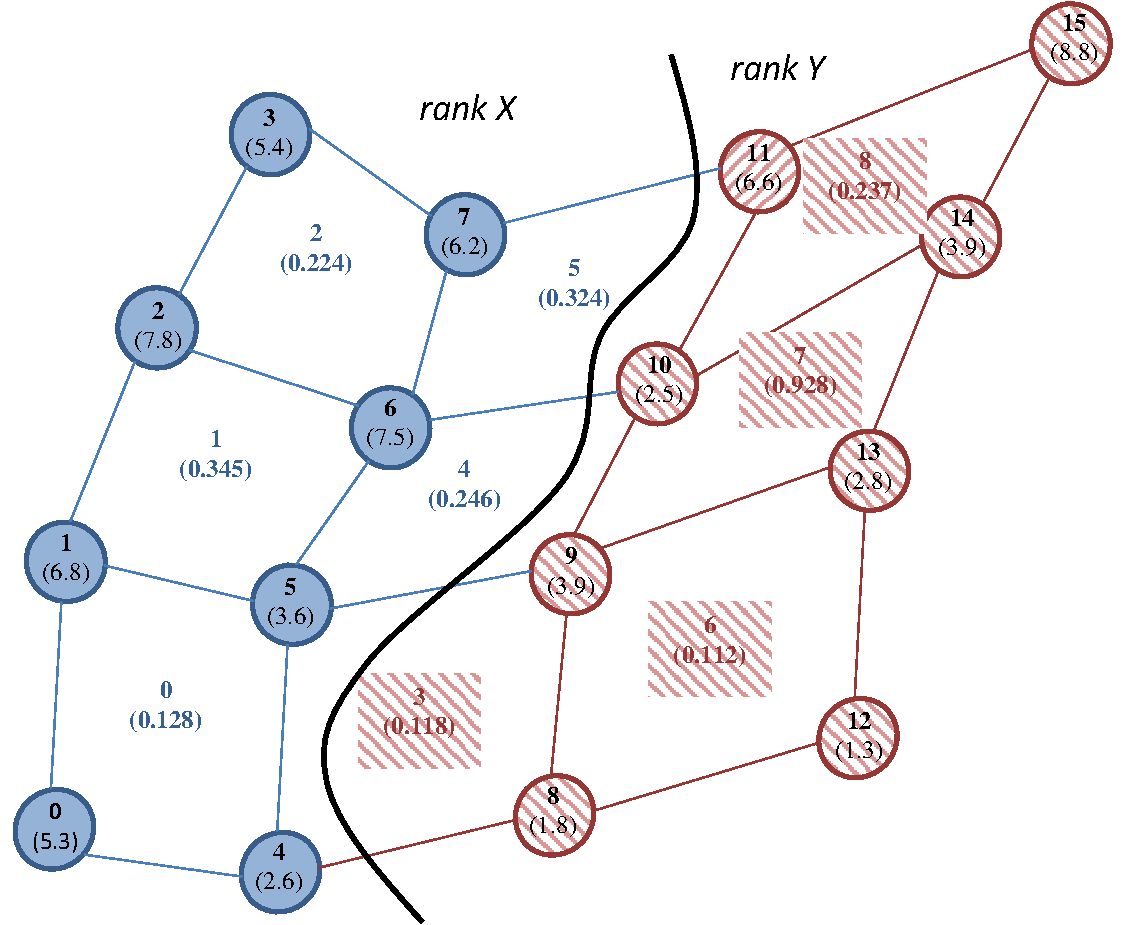
\includegraphics[width=10cm]{mesh-mpidev}\vspace{-0pt}
\caption{Example mesh with cells and nodes}\label{fig/mesh}\vspace{-10pt}
\end{figure}

\noindent In the example mesh illustrated in \figurename{ \ref{fig/mesh}} there are 16 nodes and 9 cells partitioned
across two MPI processes (rank X and rank Y). Assume that the only mapping available is a cells to node mapping. Rank X
holds nodes 0, 1, 2, 3, 4, 5, 6,and 7 and cells 0, 1, 2, 4, and 5. Rank Y holds nodes 8, 9, 10, 11, 12, 13, 14,  and 15
and cells 3, 6, 7 and 8. A loop over the cells will need data on nodes 9, 10 and 11 to be imported in to rank X from
rank Y. Additionally data on nodes 4 and 5 needs to be imported in to rank Y from rank X. On the other hand, a loop over
nodes with contributions from surrounding cells will cause cells 4 and 5 to be imported into rank Y and ``kept up to
date'' in order to receive their contributions to nodes 9, 10 and 11. Given the above scenario, each MPI process needs
to construct a list of elements for each set that needs to be
imported from and exported to other ``neighbouring'' MPI processes. Within an OP2 application, creation of these
halos occur immediately after partitioning with a call to \texttt{op\_halo\_create()}. The remainder of this section
illustrates the design and implementation of this routine and the data structures used.

\noindent In order to determine what elements of a set should be imported or exported (via MPI Send/Receives) to or from
another MPI process, we create the following classification:

\begin{itemize}
\item \textbf{CORE} : An element of a set is said to be a ``core'' element to the MPI process it is located at, if
all the elements referenced through all the mapping tables from this set element is also in the core element set in this
MPI process. e.g. In a mesh with nodes and cells (with a mapping of cells to nodes) a cell held within an MPI process is
core to this MPI process if all the nodes referenced by this cell is also core to this MPI process.

\item \textbf{Export Execute Halo (EEH)}: An element of a set is said to belong to the ``export execute halo'' if at
least one element referenced through any of the mapping tables from this set element is NOT core to this (local) MPI
process. e.g. In a mesh with nodes and cells (with a mapping of cells to nodes), if a cell references a node owned by a
foreign MPI process then this cell needs to be exported to the foreign MPI process, because it may need to be executed
on that forign process to update data on that node. This cell will fall in to the Export Execute Halo (EEH) on the local
MPI process and in turn will form part of the Import Execute Halo (IEH) on the foreign MPI process.

\item \textbf{Import Execute Halo (IEH)}: If an element of a set is referenced by an element located at a foreign MPI
process then the foreign element needs to be imported on to this MPI process in order to compute the correct
contributions to the local element. The imported element is said to be in the Import Execute Halo (IEH) of the local MPI
process. e.g. In a mesh with nodes and cells (with a mapping of cells to nodes), if a node on the local MPI process is
referenced by a cell in a foreign MPI process, then the foreign cell needs to be imported and will be part of the Import
Execute Halo (IEH) on the local MPI process.

\item \textbf{Import Non-execute Halo (INH)}: If an element located at an MPI process references (via some mapping) an
element that is located on a foreign MPI process, then the element on the foreign MPI process needs to be imported. The
imported element will fall in to the Import Non-Execute Halo (INH) if it is not already a part of the Import Execute
Halo (IEH). e.g. In a mesh with nodes and cells (with a mapping of cells to nodes), if a cell references a node owned by
a foreign MPI process then the referenced node needs to be imported onto this MPI process. The node will fall into the
Export Non-Execute Halo on the foreign MPI process.

\item \textbf{Export Non-Execute Halo (ENH)}: If an element of a set is referenced by an element located on a foreign
MPI process then the data for the local element needs to be exported on the foreign MPI process (if its not already in
the Export Execute Halo). Any loop over the foreign set element cannot proceed without getting all the contributions
from the elements it refers to. The exported element is said to be part of the Export Non-Execute Halo (ENH) on the
local MPI process. ENH is a subset of CORE. e.g. In a mesh with nodes and cells (with a mapping of cells to nodes) if a
node located on the local MPI process is referenced by a cell in a foreign MPI process, then the local node needs to be
exported to that foreign process.
\end{itemize}

\noindent The above classification allows us to clearly determine which elements of a set can be computed over without
MPI communications, facilitating overlapping of computation with communications for higher performance (see
Section~\ref{subsec/exchange}). For the mesh given in \figurename{ \ref{fig/mesh}}, the import/export elements can be
separated as follows:


\begin{table}[ht]
\centering\vspace{-10pt}
\caption{Import/Export lists}
\begin{tabular}{|c|c|c|c|c|c|} \hline
On X  & CORE        & IEH & EEH   & INH   & ENH     \\\hline
Nodes & 0, 1, 2, 3, 4, 5, 6, 7  & - & - & 8, 9, 10, 11  & 4, 5, 6, 7  \\\hline
Cells & 0, 1, 2     & 3 & 4, 5  &   &\\\hline\hline
On Y  & CORE        & IEH & EEH & INH   & ENH \\\hline
Nodes & 8, 9, 10, 11, 12, 13, 14, 15  & - & - & 4, 5, 6, 7  & 8, 9, 10, 11  \\\hline
Cells & 6, 7, 8     & 4, 5  & 3 & -   & -   \\\hline
\end{tabular}\label{tab/impexp}\vspace{-0pt}
\end{table}

\noindent The \texttt{op\_halo\_create()} routine (defined in \texttt{op\_mpi\_core.c}) goes
through all the mapping tables and creates lists that hold the indices of the set elements that fall in to the above
classification. An export or an import list for an \texttt{op\_set} has the following structure (defined in
\texttt{op\_mpi\_core.h}):

\begin{verbatim}
typedef struct {
 op_set set;        //set related to this list
 int    size;       //number of elements in this list
 int    *ranks;     //MPI ranks to be exported to or imported from
 int    ranks_size; //number of MPI neighbors
                    //to be exported to or imported from
 int    *disps;     //displacements for the starting point of each
                    //rank's element list
 int    *sizes;     //number of elements exported to or imported
                    //from each ranks
 int    *list;      //the list of all elements
} set_halo_list_core;

typedef halo_list_core* halo_list;
\end{verbatim}
\begin{verbatim}
halo_list *OP_export_exec_list;//EEH list
halo_list *OP_import_exec_list;//IEH list

halo_list *OP_import_nonexec_list;//INH list
halo_list *OP_export_nonexec_list;//ENH list
\end{verbatim}

\noindent The above four arrays are indexed using \texttt{set->index} and is of size \texttt{OP\_set\_index}. Import and
export list creation in \texttt{op\_halo\_create()} is accomplished in the following steps, by each MPI process:
\begin{enumerate}
\item \textbf{Create export lists for execute set elements}\\
Each MPI process goes through each element of each set. If a set element references (via any of the mapping table from
this set) any element that is not CORE to the local MPI process then we add the \underline{referencing} element to the
EEH list. When creating the EEH list on a given (local) MPI process, we also keep track of the foreign MPI processes
that it will be exported to. The list of elements to be sent to each foreign MPI process will be sorted according to its
local index.

\item \textbf{Create import lists for execute set elements and related mapping table entries}\\
Each MPI process exchanges the EEH list with the relevant neighbour processes and use the imported lists to
construct the IEH.

\item \textbf{Exchange mapping table entries using the import/export lists}\\
The EEH and IEH on each MPI process can now be used to exchange the bits of the mapping tables that are related to the
execute halo. The EEH and IEH of the ``from set'' of each mapping table is used to identify which mapping table entries
are to be exported and imported. For each mapping table, the imported mapping table entries will be appended to the end
of the \texttt{op\_map->map} array.

\item \textbf{Create import lists for non-execute set elements }\\
Each MPI process goes through each element of each set, (now using all the mapping table entries including the
additional mapping table entries that were imported), and adds any other element referenced (but not in IEH) to a INH
list for each set. The list of elements to be imported from each foreign MPI process will be sorted according to its
local index on the foreign process.

\item \textbf{Create non-execute set export lists}\\
Each MPI process exchanges the INH list with the relevant neighbour processes and uses the imported lists to
construct the ENH. After this step, halo lists are complete. Each MPI process has EEH, ENH, IEH and INH lists.

\item \textbf{Exchange data defined on execute set elements using the set import/ export lists}\\
The data defined on the elements belonging to each halo list is exchanged. The execute halos are exchanged first.
For each \texttt{op\_dat} the imported data will be appended to the end of the \texttt{op\_dat->data} array.

\item \textbf{Exchange data defined on non-execute set elements using the set import/export lists}\\
The non-execute halos are exchanged second. For each \texttt{op\_dat} the imported data will be appended to the end of
the \texttt{op\_dat->data} array after the IEH data.

\item \textbf{Renumber Mapping tables}\\
Each MPI process goes through all mapping table entries and renumbers the referenced set element indices to point
to local indices. All required referenced elements should be now available locally on each MPI process.

\item \textbf{Create MPI send buffers}\\
For each \texttt{op\_dat}, create some buffer space for \texttt{MPI\_Isend}s. The following struct holds the required
buffers and related data.
\begin{verbatim}
typedef struct {
 int         dat_index;    //index of the op_dat to which
                           //this buffer belongs
 char        *buf_exec;    //buffer holding exec halo
                           //to be exported;
 char        *buf_nonexec; //buffer holding nonexec halo
                           //to be exported;
 MPI_Request *s_req;       //array of MPI_Reqests for sends
 MPI_Request *r_req;       //array of MPI_Reqests for receives
 int         s_num_req;    //number of sends in flight
                           //at a given time for this op_dat
 int         r_num_req;    //number of receives awaiting
                           //at a given time for this op_dat
} op_mpi_buffer_core;

typedef op_mpi_buffer_core *op_mpi_buffer;
op_mpi_buffer *OP_mpi_buffer_list;
\end{verbatim}


\item \textbf{Separate CORE elements}\\
To facilitate overlapping of computation with communication, for each set, the CORE elements are separated to form a
contiguous block of elements. Any element NOT belonging to the EEH is a CORE element. We rearrange the local set
elements and create an \texttt{int} array (\texttt{core\_num}) holding the index that marks the end of the CORE
elements block for each set. Thus during a loop over a given set, on each MPI process, element indices \texttt{0} to
\texttt{core\_num[set->index]} can be computed over without halo data and elements from \texttt{core\_num[set->index]}
to \texttt{set->size} + \texttt{OP\_import\_exec[set->index]->size} will need to be computed over after all the calls to
\texttt{wait\_all()} are completed. See \figurename{ \ref{fig/elementorganization}}.

\begin{figure}[ht]\centering\vspace{-0pt}\hspace{10pt}
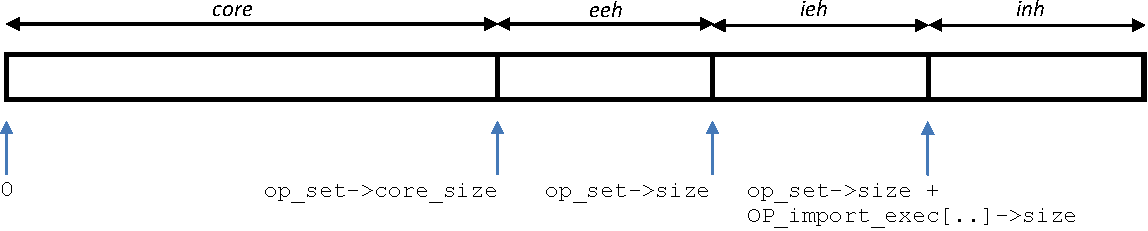
\includegraphics[width=14cm]{elementorder}\vspace{-0pt}
\caption{Element order of an \texttt{op\_set} after halo creation}\label{fig/elementorganization}\vspace{-0pt}
\end{figure}

\item \textbf{Save the original set element indices}\\
As the set elements are now rearranged, we need to keep track of the original order in which they appeared so that
calls to \texttt{op\_fetch()} and \texttt{op\_put()} as well as final outputs can be accurately handled. The
\texttt{part} struct (see Section~\ref{sec/partitioning}) is used to hold the original global indices of each set
element.

\item \textbf{Clean up and compute rough estimate of average worst-case halo size}\\
Temporary arrays are freed and a rough estimate of the average size of the worst case import halos on each MPI process
is computed. This takes in to account both the IEH and INH and accounts for the data sizes held per set element. The
calculation does NOT take in to account which halos are exchanged during the \texttt{op\_par\_loops} later in the
application.
\end{enumerate}




\noindent \figurename{ \ref{fig/elementorganization}} illustrates the element order in which data on a set will be
organized after halo creation.


% halo exchange in loops - including overlapping computation and communications
\subsection{\texttt{op\_par\_loop} and Halo Exchanges}\label{subsec/exchange}
% 1. the operation of the par_loop
A call to \texttt{op\_par\_loop} in a OP2 application executed under MPI will result in the loop being executed over
the local elements of the set on each MPI process. Additionally if the loop is an indirect loop, then computation
should be done over the IEH as well. Depending on the loop (indirect or direct) and the access type of each
\texttt{op\_arg}, halo exchanges (with a call to \texttt{exchange\_halo()}) may be needed before computation is
performed over any elements that are not CORE and in the IEH. After loop computation is performed, depending on the
access and argtype of the \texttt{op\_arg} the halos must be marked as ``dirty'' so that the next iteration of the loop
can make the decision to update the halos as required (defined in \texttt{op\_mpi\_core.c}). The current implementation
maintains a separate global \texttt{int} array that holds this information. The value \texttt{dirtybit[op\_dat->index]}
is set to 1 to indicate that the halo of \texttt{op\_dat} with index \texttt{op\_dat->index} has been modified. The
rules governing the loop operation are as follows:
\begin{enumerate}
\item If the \texttt{op\_par\_loop} consists of at least one \texttt{op\_arg} that is indirectly accessed then the
whole loop is classified as an indirect loop. Else it is a direct loop.

\item Direct loops will only need to loop over the local set size using local data and no halo exchanges are needed.

\item For indirect loops the following algorithm determines a halo exchange.
\begin{verbatim}
for each indirect op_arg {
  if ((op_arg.access is OP_READ or OP_RW) and (dirty bit is set))
  then do halo exchange for op_arg.dat and clear dirty bit
}
if(all indirect op_arg.access == OP_READ)
   execute/loop over set size
else
   execute/loop over set size + IEH
\end{verbatim}
\item After the loop computation block we set the dirty bit for each \texttt{op\_arg.dat} with \texttt{op\_arg.access}
equal to \texttt{OP\_INC, OP\_WRITE} or \texttt{OP\_RW}.
\end{enumerate}

\noindent A halo exchange is triggered by a call to \texttt{exchange\_halo(op\_set set, op\_arg arg)} which is defined
in \texttt{op\_mpi\_core.c}. Within this call, the above conditions that determines a halo exchange are checked and if
satisfied will pack the relevant halo data to the pre defined send buffers, make a call to MPI non-blocking
operations (\texttt{MPI\_Isend} and \texttt{MPI\_Irecev}) and will return 1 to indicate that a non-blocking
communication is \textit{in-flight}. As detailed in Section~\ref{subsec/halolists}, the EEH and the ENH of an MPI
process provides the indices of the elements that needs to be exported as well as the MPI ranks that will be exported
to. Using these lists an MPI process will pack the data to be set into the send buffers and then will send them using
\texttt{MPI\_Isend} operations. The following is for sending the EEH:

\begin{verbatim}
halo_list exp_exec_list = OP_export_exec_list[dat->set->index];

for(int i=0; i<exp_exec_list->ranks_size; i++) {
   for(int j = 0; j < exp_exec_list->sizes[i]; j++)
   {
     int set_elem_index = exp_exec_list->
                          list[exp_exec_list->disps[i]+j];
     memcpy(&OP_mpi_buffer_list[dat->index]->
     buf_exec[exp_exec_list->disps[i]*dat->size+j*dat->size],
     (void *)&dat->data[dat->size*(set_elem_index)],dat->size);
   }
   MPI_Isend(&OP_mpi_buffer_list[dat->index]->
          buf_exec[exp_exec_list->disps[i]*dat->size],
          dat->size*exp_exec_list->sizes[i],
          MPI_CHAR, exp_exec_list->ranks[i],
          dat->index, OP_MPI_WORLD,
          &OP_mpi_buffer_list[dat->index]->
          s_req[OP_mpi_buffer_list[dat->index]->s_num_req++]);
  }
\end{verbatim}
\noindent The \texttt{MPI\_Isend} operations are immediately followed by \texttt{MPI\_Irecev} operations, which sets up
the non-blocking communications to directly copy the incoming data in to the relevant \texttt{op\_dat}, using the IEH
and INH lists.
\begin{verbatim}
halo_list imp_exec_list = OP_import_exec_list[dat->set->index];

int init = dat->set->size*dat->size;
for(int i=0; i < imp_exec_list->ranks_size; i++) {
   MPI_Irecv(&(OP_dat_list[dat->index]->
          data[init+imp_exec_list->disps[i]*dat->size]),
          dat->size*imp_exec_list->sizes[i],
          MPI_CHAR, imp_exec_list->ranks[i],
          dat->index, OP_MPI_WORLD,
          &OP_mpi_buffer_list[dat->index]->
          r_req[OP_mpi_buffer_list[dat->index]->r_num_req++]);
}
\end{verbatim}

\noindent A call to \texttt{wait\_all(op\_arg arg)} routine needs to be performed in order to complete the MPI
communications. The \texttt{op\_par\_loop} is structured so that all the \texttt{exchange\_halo()} calls are done at the
beginning of the loop, followed by computation over the CORE elements of the set and then by calls to
\texttt{wait\_all()}. This will allow for maximum overlapping of computation with communication as none of the CORE
elements reference any halo data. After the calls to \texttt{the wait\_all()} the remaining set elements could be
computed. A reference implementation of the above can be found in \texttt{op\_mpi\_seq.h}.

% global operations
\subsection{Global Operations}\label{subsec/globalops}

If an \texttt{op\_arg} is of type \texttt{OP\_ARG\_GBL} then a global operation needs to be performed for that
argument. The operation to be performed is one of \texttt{OP\_INC} (global reduction), \texttt{OP\_MAX} (global
maximum), \texttt{OP\_MIN} (global minimum). For an \texttt{op\_arg} of type \texttt{OP\_ARG\_GBL}, the contributions
from executing the IEH must not be included Thus the reference implementation passes in a dummy value in place of any
\texttt{op\_arg} with type \texttt{OP\_ARG\_GBL}. After the loop over the elements are performed on each MPI process,
the global operation should be done across all the MPI processes by a call to \texttt{global\_reduce()} which is also
defined in \texttt{op\_mpi\_core.c}. This routine checks for the type of the data exchanged and the type of the
operation to be performed and calls \texttt{MPI\_Reduce} with the relevant operation and data type.

% implementing op_fetch and op_put
\subsection{\texttt{op\_fetch\_data} }\label{subsec/putfetch}
The proposed operation of \texttt{op\_fetch\_data (op\_dat dat)} within an OP2 application executing over MPI will be to
present the current values of the \texttt{op\_dat}'s data array in the order of the elements that was originally handed
to OP2. It should be noted that the data array presented to the user level application is a \underline{copy} of the
current state of the internal \texttt{op\_dat}. This routine is currently not implemented. A valid implementation will
first make a copy of the current data values in the \texttt{op\_dat} requested and will reorder them according to the
original global index of the set elements on which this data is defined on.

Conversely an \texttt{op\_put\_data()} routine may also be implemented (as required) so that the user level application
can modify the internal values of an \texttt{op\_dat}. In this case the user submitted data values will replace the
internal \texttt{op\_dat}'s data values. A valid implementation will need to translate the original set element index
to the current set element index.


% debug routines
\subsection{Debug Routines}\label{subsec/debug}
Currently only one debug routine is used, \texttt{reset\_halo(op\_arg arg)}, which initialise import
halo data to NaN - for diagnostics purposes. If \texttt{OP\_diags} is $>$ 2 then this routine is called to reset a halo
for each \texttt{op\_arg}.

% performance measurements - including flags to trigger them
\subsection{Performance Measurements}\label{subsec/perf}
The time spent in the \texttt{op\_par\_loop()} calls is measured and accumulated. The setup costs due to halo creation
and partitioning are also measured and the maximum on all the processors is printed to standard out by rank 0.
Additionally information about the amount of MPI communications performed is also collected. For each
\texttt{op\_par\_loop()} we maintain a struct that holds (1) the accumulated time spent in the loop (2) the number of
times the \texttt{op\_par\_loop()} routine is called, (3) the indices of the \texttt{op\_dat}s that requires halo
exchanges during the loop, (4) the total number of times halo exchanges are done for each \texttt{op\_dat} and (5)
the total number of bytes exported for each \texttt{op\_dat}.
\begin{verbatim}
typedef struct
{
  char const  *name;   // name of kernel
  double      time;    //total time spent in this
                       //kernel (compute+comm-overlapping)
  int         count;   //number of times this kernel is called
  int*        op_dat_indices;  //array to hold op_dat index of
                               //each op_dat used in MPI halo
                               //exports for this kernel
  int         num_indices; //number of op_dat indices
  int*        tot_count;   //total number of times this op_dat was
                           //halo exported within this kernel
  int*        tot_bytes;   //total number of bytes halo exported
                           //for this op_dat in this kernel
} op_mpi_kernel;
\end{verbatim}
\noindent Currently, the only way to identify a loop is by its name. Thus we use a simple hash function on the
name string to index into a hash table (\texttt{op\_mpi\_kernel\_tab[]}) that holds an \texttt{op\_mpi\_kernel} struct
for each loop. Monitoring the halo exchanges require calls to the \texttt{op\_mpi\_perf\_comm()} (defined in
\texttt{op\_mpi\_core.c}) for each \texttt{op\_arg} that has had a halo exchanged during each call to an
\texttt{op\_par\_loop()}. As this may cause some performance degradation, we allow the MPI message monitoring to be
enabled at compile time using the \texttt{-DCOMM\_PERF} switch.



% output routines
\subsection{Output Routines}\label{subsec/output}
A number of output routines are provided currently, including routines to output the performance measures,
\texttt{op\_mpi\_timing\_output()} as well as file writes that directly writes an \texttt{op\_dat} to an ASCI file,
\texttt{gatherprint\_tofile()} or a binary file, \texttt{gatherprint \_bin\_tofile()}. These routines gathers a
specified
\texttt{op\_dat}, (which is distributed across the MPI universe) on to MPI rank 0 and prints the results to a user
specified file. The \texttt{op\_dat} will be written to file in the same order in which the set elements were handed to
OP2 during the initial input of data and mapping tables. This requires calls to \texttt{op\_fetch()}.

% clean-up routines
\subsection{Garbage Collection}\label{subsec/cleanup}
At the end of the OP2 application a call to \texttt{op\_halo\_destroy()} will free all halo lists, MPI send buffers and
the table holding performance measures.

\newpage
\section{Partitioning}\label{sec/partitioning}
Given the unstructured mesh in an OP2 application, distributing the data on sets and mapping tables across the MPI
universe is achieved by a mesh partitioner in order to avoid building large halos. The OP2 proposal is to
achieve good partitions without the intervention of the application programmer. The idea is that once the OP2
declaration routines are executed the MPI back-end should call a partitioning routine to partition the sets and maps and
migrate the data to new MPI processes as required. There are a number of grid/mesh partitioners that can be
used for this task, however at the moment it is not clear which one will provide the best performance. The current
distributed memory implementation gives the option of using either (1) a geometric partitioning, (2) k-way graph
partitioning with ParMetis~\cite{ParMETIS} or (3) k-way graph partitioning with PT-Scotch. OP2 also provides a number of
supporting functions and data migration routines to facilitate the above goals. However, a number of extensions need to
be implemented to obtain high quality partitions as well as to make the partitioning truly seamless with no user
intervention at the application program level.\\
\indent The OP2 proposal is to partition the mesh immediately after all the calls to \texttt{op\_decl\_*}. Thus we
assume that an initial parallel distribution of the sets and mapping tables has been performed during input, either by
user defined I/O routines or using the HDF5 parallel I/O routines. For example in the \texttt{airfoil\_mpi} application
the data and mappings are distributed in a block partitioning fashion. The partitioning of the sets are performed by
calls to wrapper functions: \texttt{op\_partition\_geom()}, \texttt{op\_partition\_kway()} or
\texttt{op\_partition\_ptscotch()} defined in \texttt{op\_mpi\_part\_core.c}. A wrapper functions are required to
organize the data and/or mesh elements into a format that is acceptable to the ParMetis and PT-Scotch partitioning
routines. We anticipate that supporting further different partitioners may require other wrapper functions to be
developed into the MPI back-end. A future proposal is to provide decision logic that selects the appropriate partitioner
routine (by calling the appropriate wrapper function) depending on the available \texttt{op\_set}s, \texttt{op\_map}s
and \texttt{op\_dat}s without the intervention of the application programmer.\\
\indent For example in the airfoil application, the xy coordinates of the nodes are supplied in \texttt{p\_x}. Thus
\texttt{op\_partition\_geom()} can be utilized with \texttt{p\_x}. After a call to \texttt{op\_partition\_geom()}, on
each MPI process, the ParMetis routine returns an array that gives the new MPI rank of each set element (in this case
for each node). At this point of the application we consider nodes as the \underline{partitioned} (primary) set. The
primary set and the available mapping tables will now allow to partition all other sets. These secondary sets will
\textit{inherit} the primary set's partitioning. Partitioning secondary sets is achieved by a call to
\texttt{partition\_all()} from within a wrapper function. Next, a call to \texttt{migrate\_all()} migrates the data and
mappings to the new MPI process and will sort the elements on the new MPI ranks.  Finally \texttt{renumber\_maps()}
will renumber mapping table entries with new indices. \\
\indent At the end of an OP2 application, the partitioning needs to be reversed in order to revert back to the original
set element order in which the user application supplied the data on sets and mapping tables to OP2. This is achieved in
\texttt{op\_partition\_reverse()} where the original partition information (which was saved during the partition
creation and halo creation routines) are used to reverse the mapping table renumbering and migrate the data on sets to
their original MPI rank and sort them in the original element index order. \\

\noindent For debugging purposes, we have also implemented a wrapper function: \texttt{op\_partition\_ random()} that
performs a random partitioning of a given set.


\section{To do list}
\begin{itemize}
\item Design/implement OP2 to use CUDA/OpenMP within a node on top of the current MPI implementation
\item Provide decision logic that selects the appropriate partitioner routine depending on the available
\texttt{op\_set}s, \texttt{op\_map}s and \texttt{op\_dat}s without the intervention of the application programmer.
\item Design and implement HDF5 file IO - define input file format
\item Implement automatic check-pointing
\end{itemize}


% do we need to rethink the partitioning given the HDF5 I/O ? - need to hid the partitioning behind the scenes

\begin{thebibliography}{9}

\bibitem{ParMETIS} ParMETIS user manual,\\http://glaros.dtc.umn.edu/gkhome/fetch/sw/parmetis/manual.pdf
\bibitem{PTScotch} Scotch and PTScotch,\\http://www.labri.fr/perso/pelegrin/scotch/


\end{thebibliography}



\end{document}


\begin{comment}
 The following struct supports the partitioning of set elements. At the end of the partitioning it will hold the
original(pre-partitioning) global indices of each set element, to facilitate the revere partitioning.
typedef struct
{
  op_set set;    //set to which this partition info blongs to
  int *g_index;  //global index of each element held in
                 //this MPI process
  int *elem_part;//partition(MPI rank) to which each
                 //element belongs
  int is_partitioned; //indicates if this set is partitioned
                      //1 if partitioned 0 if not
} part_core;

typedef part_core *part;
\end{comment}


